\documentclass[10pt]{article}
\usepackage[margin=0.56in]{geometry}
\usepackage{booktabs,enumitem,fancyhdr,graphicx,tabularx,titlesec}
\usepackage[table]{xcolor}
\usepackage[hidelinks]{hyperref}
\graphicspath{{docs/lessons/assets/}{../assets/}}
\hypersetup{pdftitle={ADK Lesson 050: Bounded Logical Homing},
 pdfauthor={Kevin Shanahan},
 pdfsubject={Copied home evidence, bounded homing, volatile logical position, and inert step intent},
 pdflang={en-US}}
\pagestyle{fancy}\fancyhf{}
\lhead{\textsc{ADK Lesson 050}}\rhead{Bounded Logical Homing}
\cfoot{\thepage}\setlength{\headheight}{14pt}
\setlength{\parindent}{0pt}\setlength{\parskip}{1.5pt}
\setlist{nosep,leftmargin=1.45em}
\titleformat{\section}{\Large\bfseries}{\thesection}{0.5em}{}
\titlespacing*{\section}{0pt}{7pt}{2pt}
\titlespacing*{\subsection}{0pt}{5pt}{2pt}
\newcommand{\lessonbox}[1]{\begin{center}\fbox{\parbox{0.92\linewidth}{#1}}\end{center}}
\newcommand{\blankline}{\rule{0.72in}{0.4pt}}

\begin{document}
\small
\begin{center}
 {\Huge\bfseries Bounded Logical Homing}\\[3pt]
 {\Large Release, seek, and establish one volatile origin}\\[7pt]
 \fbox{\textbf{E0 COPIED REPLAY --- NO SENSOR, COIL, MOTOR, OR POSITION CLAIM}}
\end{center}
\begin{tabularx}{\linewidth}{@{}>{\bfseries}l X >{\bfseries}l X@{}}
Lesson & 050 --- component & Time & 110--160 minutes\\
Prerequisite & Lesson 047 & Board & compile-only Mega replay\\
Evidence & named memory result cells & Position & volatile logical fixture only\\
\end{tabularx}

\lessonbox{\textbf{Component boundary.} \texttt{BoundedHomingPolicy} converts
copied, already-qualified home and independent-stop evidence into at most one
signed semantic step request per accepted frame. It owns no pin, timer,
interrupt, bus, sensor, sequencer, coil vector, driver, supply, callback,
heap allocation, or physical position.}

\section{Begin with position unknown}
Initialization publishes \texttt{PositionUnknown}, asserts software stop
intent, clears the step request, and establishes no home epoch. A caller must
explicitly request homing. Reset, shutdown, restart, source failure, or
interrupted logical travel cannot restore an earlier position.

\begin{tabularx}{\linewidth}{@{}l X@{}}
\toprule
Configuration field & E0 rule\\
\midrule
logical bounds & inclusive negative and positive bounds around zero\\
search direction & exactly \(-1\) or \(+1\)\\
release/search limits & separate nonzero step and duration bounds\\
step cadence & nonzero; delayed calls never burst or catch up\\
copied evidence & bounded freshness and input skew; stable provenance\\
\bottomrule
\end{tabularx}

The home coordinate is exactly zero. Invalid, unrepresentable,
half-range-ambiguous, zero-duration, or internally inconsistent configuration
is rejected before the policy starts. These are integer and replay
constraints, not mechanical dimensions.

\section{Release first, then acquire an edge}
\begin{center}
% ADK visual: pencil
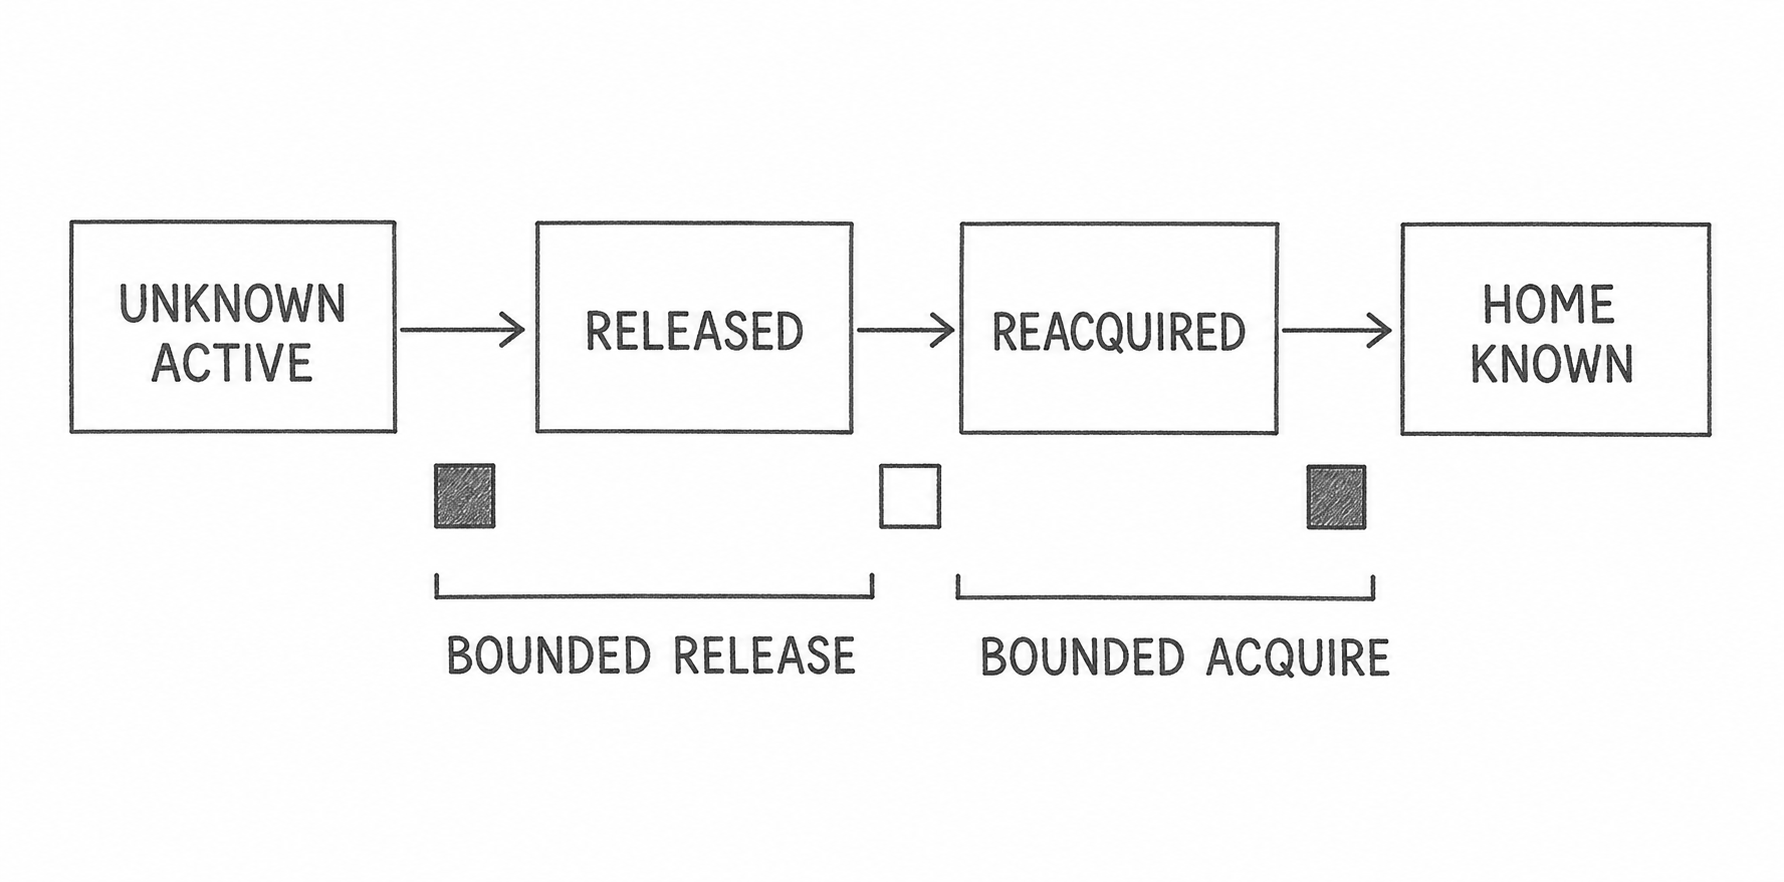
\includegraphics[width=0.96\linewidth,height=0.29\textheight,
 keepaspectratio]{050-release-acquire-pencil.png}

\small\textit{Alternative text: a graphite-pencil timeline shows an initially
active copied home record moving through bounded release, bounded search, a
new qualified inactive-to-active edge, and logical zero. Separate rulers mark
release and search limits; no wiring or physical mechanism is depicted.}
\end{center}

An active level at startup is ambiguous. It could represent a carriage at
home, a broad target encountered elsewhere, reversed polarity, or a stuck
sensor. Therefore an initial active record is never accepted as home.

\begin{enumerate}
 \item Admit one structurally valid, qualified copied home observation.
 \item If it is active, enter \texttt{SeekingHomeRelease} and request bounded
       signed steps opposite the configured search direction.
 \item Accept only a qualified inactive release from the same evidence domain.
 \item Enter \texttt{SeekingHome} and request bounded steps in the configured
       search direction.
 \item Accept home only on a new qualified inactive-to-active edge.
 \item Clear step intent before publishing position zero and a nonzero home
       epoch.
\end{enumerate}

An initially inactive observation begins directly in \texttt{SeekingHome}.
The initial sample, release, and acquisition edge retain the same source kind,
source ID, configuration revision, and nonzero qualification epoch. A held
active level is not a new edge, and an unqualified inactive value is not a
release.

\section{Keep release and search bounds independent}
Release and approach each have their own issued-step limit and elapsed-time
limit. The exact configured boundary is accepted; only the next frame fails.
Exhausting release yields \texttt{HomeStuckActive}. Exhausting search without
the qualified edge yields \texttt{HomeNotFound}. Neither retries
automatically.

\begin{tabularx}{\linewidth}{@{}l X X@{}}
\toprule
Phase & Accepted evidence & Terminal failure\\
\midrule
\texttt{SeekingHomeRelease} & qualified inactive release & stuck active\\
\texttt{SeekingHome} & qualified inactive-to-active edge & home not found\\
\texttt{Homed} & bounded target and healthy frames & stop or admitted fault\\
\bottomrule
\end{tabularx}

One accepted update emits at most one due signed request. A delayed call does
not create a burst and does not infer skipped physical movement. The policy
advances only its own logical fixture coordinate after its request is
accepted; it cannot observe an applied motor step.

\section{Preview the whole transition, then commit once}
Every candidate update is side-effect free until committed.
\texttt{preview()} checks the complete copied frame, command, provenance,
time, arithmetic, and transition. \texttt{canCommit()} proves that the
candidate belongs to the unchanged policy generation. \texttt{commit()} then
publishes one complete \texttt{HomingSnapshot}.

\begin{tabularx}{\linewidth}{@{}l X@{}}
\toprule
Snapshot field & Meaning at E0\\
\midrule
\texttt{logicalPosition} & volatile fixture coordinate\\
\texttt{positionKnown} & this session accepted a synthetic home edge\\
\texttt{stepRequested} & one semantic request is due\\
\texttt{requestedStepDirection} & \(-1\) or \(+1\), never a coil vector\\
\texttt{stopIntent} & software request to inhibit downstream motion\\
\texttt{homingSteps} & bounded requests issued in this home attempt\\
\texttt{homeEpoch} & nonzero identity of the current session-local result\\
\bottomrule
\end{tabularx}

A foreign, stale, changed, replayed, or consumed preview rejects without
mutation. Lesson 051 may jointly preflight this semantic candidate with its
separately owned Lesson 047 sequencer. Lesson 050 neither contains nor calls
that sequencer.

\section{Travel only inside the logical excursion}
\begin{center}
% ADK visual: pencil
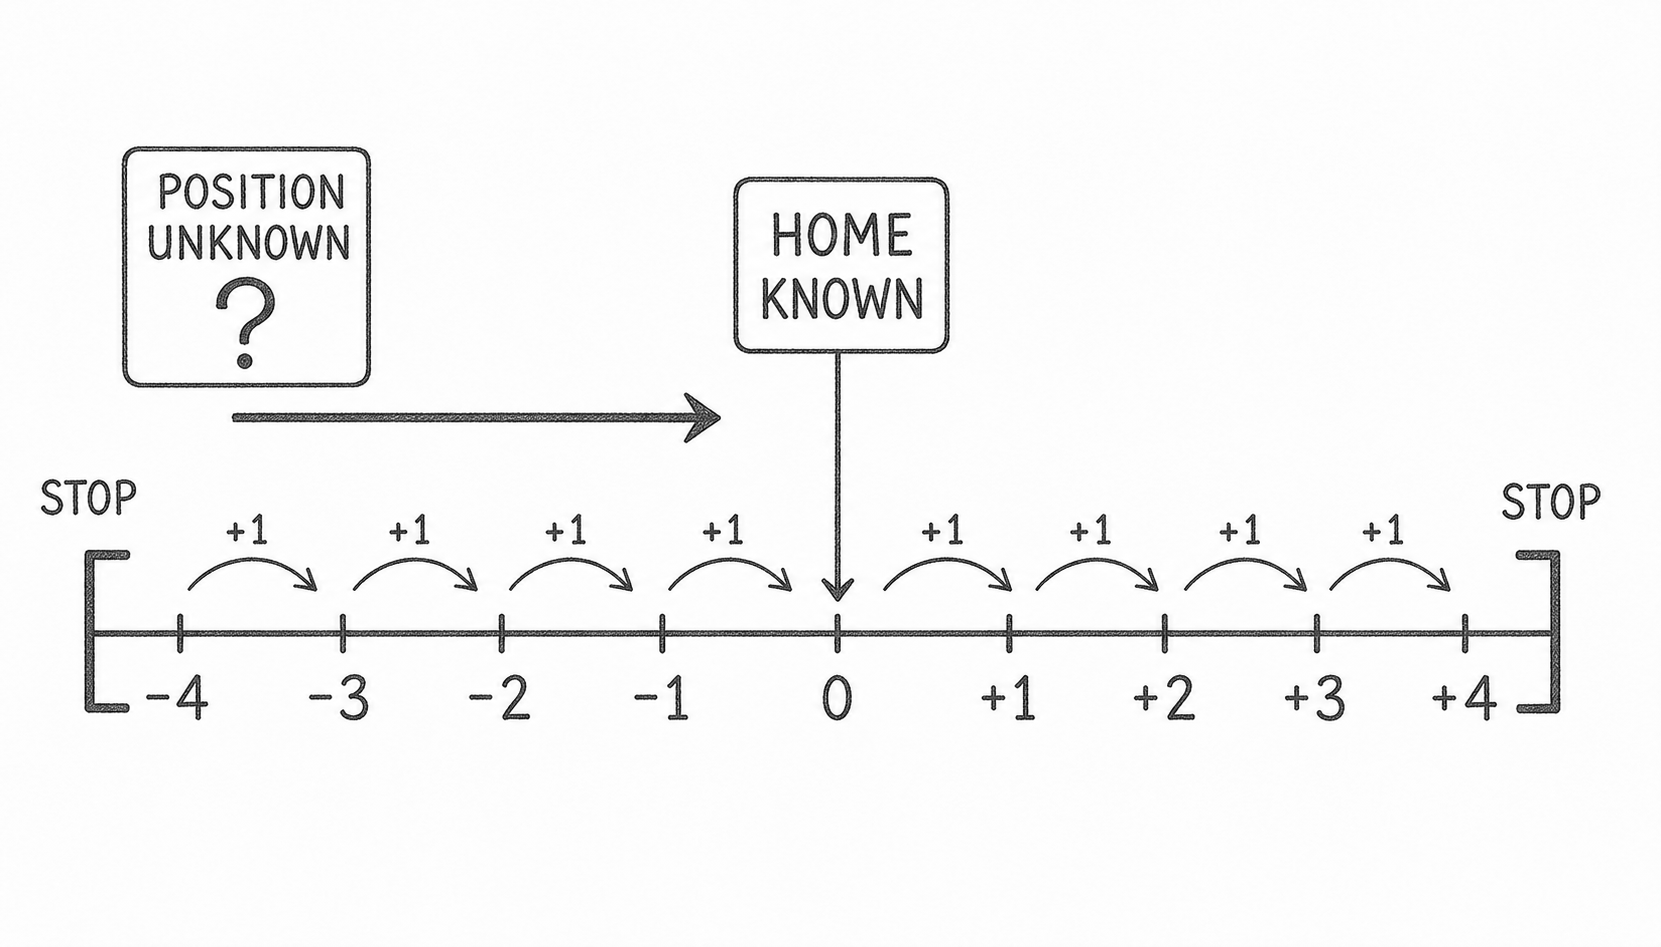
\includegraphics[width=0.94\linewidth,height=0.25\textheight,
 keepaspectratio]{050-logical-bounds-pencil.png}

\small\textit{Alternative text: a rough pencil number line places volatile
logical zero between inclusive negative and positive bounds. An unknown-state
card is separate from the line. The drawn \(+1\) arrows illustrate one-step
travel in the positive direction; the policy issues signed \(-1\) or \(+1\)
requests and stops at either inclusive boundary.}
\end{center}

Only a homed session accepts a target. The target must lie inside the
inclusive configured bounds. A zero-distance command completes without a
step; otherwise each due accepted frame publishes one signed request until
the logical fixture reaches the target.

Checked subtraction precedes addition at every signed boundary. The immutable
\texttt{excursionBounds()} result covers zero and the largest release and
search excursions without narrowing before representability is proven. This
proves bounded arithmetic, not shaft motion, measured travel, switch
activation, or motor shutdown.

\section{Let independent stop dominate}
A separately admissible, qualified active stop dominates every ordinary
request, evidence fault, due step, acquisition edge, final step, and target.
It clears the request and asserts stop intent in the same commit, even when
unrelated home or command fields are malformed.

If stop interrupts homing or logical travel, the policy enters
\texttt{Stopped} and forgets position. A stop while idle in \texttt{Homed}
may retain the known logical coordinate because no displacement was in
progress. After release, recovery still requires an explicit command; no
held or released level starts motion.

A malformed stop channel cannot be trusted inactive, so complete-frame
rejection wins. Other admitted source or motion failures enter
\texttt{Fault}, assert stop intent, and invalidate the home epoch. Fault
recovery requires shutdown followed by initialization. Software stop intent
is not an emergency stop, removed motor power, or electrical safe-state proof.

\section{Run the deterministic E0 workbook}
\begin{enumerate}
 \item Initialize. Predict unknown position, asserted stop intent, no step,
       and zero home epoch.
 \item Start homing with copied home active. Predict bounded release requests
       opposite search; repeat an active level and confirm it is not an edge.
 \item Supply a qualified inactive release, then due search frames. Predict
       at most one search request per accepted frame.
 \item Supply a new qualified active edge at the exact search bound. Predict
       \texttt{Homed}, logical zero, cleared step request, and a new epoch.
 \item Request each inclusive logical bound, then zero distance. Record signed
       requests and completion without claiming applied motion.
 \item Exhaust release and search independently. Distinguish
       \texttt{HomeStuckActive} from \texttt{HomeNotFound}.
 \item Collide an active valid stop with a due step and malformed unrelated
       evidence. Predict \texttt{Stopped}, no step, and asserted stop intent.
 \item Inject provenance change, source fault, same-time changed evidence,
       rollover ambiguity, restart, and shutdown. Predict atomic rejection or
       the specified unknown-position terminal state.
\end{enumerate}

\subsection*{E0 result cells}
\begin{tabularx}{\linewidth}{@{}X X X X X@{}}
\toprule
frame & phase & known? & logical position & home epoch\\
\midrule
\rule{0pt}{16pt}\blankline & \blankline & \blankline & \blankline & \blankline\\[9pt]
\blankline & \blankline & \blankline & \blankline & \blankline\\[9pt]
\blankline & \blankline & \blankline & \blankline & \blankline\\
\bottomrule
\end{tabularx}

\begin{tabularx}{\linewidth}{@{}X X X X X@{}}
\toprule
source/sequence & home level & requested step & stop intent & status\\
\midrule
\rule{0pt}{16pt}\blankline & \blankline & \blankline & \blankline & \blankline\\[9pt]
\blankline & \blankline & \blankline & \blankline & \blankline\\[9pt]
\blankline & \blankline & \blankline & \blankline & \blankline\\
\bottomrule
\end{tabularx}

\section{Interpret only what E0 observes}
\textbf{Acquisition prediction.} Qualified copied evidence with consistent
source, revision, epoch, sequence, time, polarity, and status can form the
release and acquisition history.

\textbf{Acquisition observation.} Executable host tests inspect the copied
records, phase, request direction, logical position, epoch, stop intent, and
status in memory.

\textbf{Acquisition interpretation.} A successful replay proves a pure
copied-data transition and a session-local fixture origin. It does not prove
that a switch, pin, clock, sensor, carriage, or origin was acquired.

\textbf{Safe-state prediction.} Stop, fault, interrupted motion, reset, and
shutdown clear the step request, assert stop intent where specified, and
invalidate position when displacement cannot be established.

\textbf{Safe-state observation.} Inspect the complete committed snapshot and
retained terminal attribution.

\textbf{Safe-state interpretation.} An inert memory result proves only policy
precedence. It does not prove de-energized coils, stationary hardware, a dark
indicator, or independent removal of actuator power.

\section{Keep the resource claim bounded}
The canonical Mega replay uses fixed storage, bounded O(1) work, and no heap
or hardware resource. Promotion requires the \texttt{BoundedHomingPolicy}
object to remain at or below 128 bytes (measured: 126 bytes), the sketch to
remain within 16,384 bytes flash and 1,024 bytes static SRAM (measured: 8,272
and 574 bytes), at least 448 bytes of conservative stack/ISR allowance, and at
least 768 bytes remaining after globals and that allowance.

\lessonbox{\textbf{Compile-only means compile-only.} Packaging proves that
the public API, fixture, and named result schema fit the Mega build. It does
not execute the fixture or prove a powered board populated any result cell.}

\section{Leave E1 copied-input acceptance blank}
\lessonbox{\textbf{E1 remains open.} E1 may qualify exact low-energy home and
stop producers plus a non-motion observation path. It cannot establish
physical home or energize a motor.}

\begin{tabularx}{\linewidth}{@{}>{\bfseries}l X@{}}
Exact sensor and stop specimens & \rule{0pt}{16pt}\hrulefill\\[9pt]
Primary datasheets and revision markings & \hrulefill\\[9pt]
Supply, logic levels, polarity, and pin order & \hrulefill\\[9pt]
Qualification, release, edge, and bounce evidence & \hrulefill\\[9pt]
Named LED/display/test-point observation path & \hrulefill\\[9pt]
Fault, disconnect, reset, and rollback observation & \hrulefill\\[9pt]
Reviewer, date, acceptance record & \hrulefill\\
\end{tabularx}

\section{Leave E2 powered homing acceptance blank}
\lessonbox{\textbf{E2 remains open.} No physical build is authorized until
the exact sensor, motor, driver, supply, mechanism, protection, and independent
power-removal path are identified and reviewed together.}

\begin{tabularx}{\linewidth}{@{}>{\bfseries}l X@{}}
Exact motor, winding, driver, and sensor & \rule{0pt}{16pt}\hrulefill\\[9pt]
Electrically authoritative schematic review & \hrulefill\\[9pt]
Current-limited actuator supply and common & \hrulefill\\[9pt]
Measured coil, aggregate, and thermal limits & \hrulefill\\[9pt]
Restraint, pinch guarding, and overtravel margin & \hrulefill\\[9pt]
Release, search, stall, and collision measurements & \hrulefill\\[9pt]
Independent stop and actuator-power removal & \hrulefill\\[9pt]
Recorded physical homing acceptance result & \hrulefill\\[9pt]
Reviewer, date, acceptance record & \hrulefill\\
\end{tabularx}

Future E2 work is limited to a lightweight stable tabletop mechanism with no
loose load, sharp or high-inertia feature, stored energy, lifting, vehicle,
door-lock, launcher, or safety-device role. Firmware stop intent and a
software home epoch cannot substitute for restraint or independently removed
power.

\section{Software evidence and further work}
Deterministic tests cover inactive and active starts, bounded release and
search, qualification and provenance, exact limits and deadlines, missing
and stuck home, bounded targets, preview lifetime, stop and fault collisions,
rollover, interruption, recovery, shutdown, and byte-stable replay.

\begin{itemize}
 \item \href{https://github.com/spincyc/adk/blob/main/examples/Lesson050BoundedHomingPolicy/Lesson050BoundedHomingPolicy.ino}
       {Canonical compile-only Lesson 050 sketch}.
 \item \href{https://github.com/spincyc/adk/blob/main/tests/test_bounded_homing_policy.cpp}
       {Deterministic bounded-homing tests}.
 \item \href{https://github.com/spincyc/adk/blob/main/src/bounded_homing_policy.h}
       {Bounded-homing interface}.
 \item \href{https://github.com/spincyc/adk/blob/main/docs/design/LESSONS_049_051_PARTS_CAROUSEL_PLAN.md}
       {Lessons 049--051 design record}.
 \item \href{https://github.com/spincyc/adk/blob/main/docs/TESTING.md}
       {Deterministic testing contract}.
 \item \href{https://github.com/spincyc/adk/blob/main/docs/SAFETY_MODEL.md}
       {Safety model}.
\end{itemize}

This untagged print edition has a searchable HTML alternative.
It makes no PDF/UA, powered-input, motion, or physical-position claim.
\end{document}
